\documentclass[11pt,openany]{article}

\usepackage{mathtools, commath}
% Packages for formatting
\usepackage[margin=1in]{geometry}
\usepackage{fancyhdr}
\usepackage{enumerate}
\usepackage{graphicx}
\usepackage{kotex}
\usepackage{arydshln} % Include this package
\usepackage{bbding}
\usepackage{amsmath}
\usepackage{amsthm}
\usepackage[dvipsnames,table]{xcolor}
\usepackage{amssymb, amsfonts}
\usepackage{wasysym}
\usepackage{footnote}
\usepackage{tablefootnote}
\usepackage{arydshln} % Include this package
% Fonts
\usepackage[T1]{fontenc}
\usepackage[utf8]{inputenc}
\usepackage{newpxtext,newpxmath}
\usepackage{sectsty}

% Define colors
\definecolor{TealBlue1}{HTML}{0077c2}
\definecolor{TealBlue2}{HTML}{00a5e6}
\definecolor{TealBlue3}{HTML}{b3e0ff}
\definecolor{TealBlue4}{HTML}{00293c}
\definecolor{TealBlue5}{HTML}{e6f7ff}

\definecolor{thmcolor}{RGB}{231, 76, 60}
\definecolor{defcolor}{RGB}{52, 152, 219}
\definecolor{lemcolor}{RGB}{155, 89, 182}
\definecolor{corcolor}{RGB}{46, 204, 113}
\definecolor{procolor}{RGB}{241, 196, 15}

\usepackage{color,soul}
\usepackage{soul}
\newcommand{\mathcolorbox}[2]{\colorbox{#1}{$\displaystyle #2$}}
\usepackage{cancel}
\newcommand\crossout[3][black]{\renewcommand\CancelColor{\color{#1}}\cancelto{#2}{#3}}
\newcommand\ncrossout[2][black]{\renewcommand\CancelColor{\color{#1}}\cancel{#2}}

\usepackage{hyperref}
\usepackage{booktabs}

% Chapter formatting
\definecolor{titleTealBlue}{RGB}{0,53,128}
\usepackage{titlesec}
\titleformat{\section}
{\normalfont\sffamily\Large\bfseries\color{titleTealBlue!100!gray}}{\thesection}{1em}{}
\titleformat{\subsection}
{\normalfont\sffamily\large\bfseries\color{titleTealBlue!50!gray}}{\thesubsection}{1em}{}

%Tcolorbox
\usepackage[most]{tcolorbox}
\usepackage{multirow}
\usepackage{multicol}

\usepackage[linesnumbered,ruled]{algorithm2e}
\usepackage{algpseudocode}
\usepackage{setspace}
\SetKwComment{Comment}{/* }{ */}
\SetKwProg{Fn}{Function}{:}{end}
\SetKw{End}{end}
\SetKw{DownTo}{downto}

% Define a new environment for algorithms without line numbers
\newenvironment{algorithm2}[1][]{
	% Save the current state of the algorithm counter
	\newcounter{tempCounter}
	\setcounter{tempCounter}{\value{algocf}}
	% redefine the algorithm numbering (remove prefix)
	\renewcommand{\thealgocf}{}
	\begin{algorithm}
	}{
	\end{algorithm}
	% Restore the algorithm counter state
	\setcounter{algocf}{\value{tempCounter}}
}

\usepackage{adjustbox}
% Header and footer formatting
\pagestyle{fancy}
\fancyhead{}
\fancyhf{}
\rhead{\textcolor{TealBlue2}{\large\textbf{기대수(기초부터 대학원 수학까지 시리즈) 3기}}}%\rule{3cm}{0.4pt}}
\lhead{\textcolor{TealBlue2}{\large\textbf{수학의 즐거움, Enjoying Math}}}
% Define footer
%\newcommand{\footer}[1]{
%\begin{flushright}
%	\vspace{2em}
%	\includegraphics[width=2.5cm]{school_logo.jpg} \\
%	\vspace{1em}
%	\textcolor{TealBlue2}{\small\textbf{#1}}
%\end{flushright}
%}
%\rfoot{\large Department of Information Security, Cryptogrphy and Mathematics, Kookmin Uni.\includegraphics[height=1.5cm]{school_logo.jpg}}
\fancyfoot{}
\fancyfoot[C]{-\thepage-}

\usepackage{tcolorbox}
\tcbset{colback=white, arc=5pt}

\definecolor{axiomcolor}{HTML}{a88bfa}
\definecolor{defcolor}{RGB}{52, 152, 219}
\definecolor{procolor}{RGB}{241, 196, 15}
\definecolor{thmcolor}{RGB}{231, 76, 60}
\definecolor{lemcolor}{RGB}{155, 89, 182}
\definecolor{corcolor}{RGB}{46, 204, 113}
\definecolor{execolor}{RGB}{90, 128, 127}

% Define a new command for the custom tcolorbox
\newcommand{\axiombox}[2][]{%
	\begin{tcolorbox}[colframe=axiomcolor, title={\color{white}\bfseries #1}]
		#2
	\end{tcolorbox}
}

\newcommand{\defbox}[2][]{%
	\begin{tcolorbox}[colframe=defcolor, title={\color{white}\bfseries #1}]
		#2
	\end{tcolorbox}
}

\newcommand{\lembox}[2][]{%
	\begin{tcolorbox}[colframe=lemcolor, title={\color{white}\bfseries #1}]
		#2
	\end{tcolorbox}
}

\newcommand{\probox}[2][]{%
	\begin{tcolorbox}[colframe=procolor, title={\color{white}\bfseries #1}]
		#2
	\end{tcolorbox}
}

\newcommand{\thmbox}[2][]{%
	\begin{tcolorbox}[colframe=thmcolor, title={\color{white}\bfseries #1}]
		#2
	\end{tcolorbox}
}

\newcommand{\corbox}[2][]{%
	\begin{tcolorbox}[colframe=corcolor, title={\color{white}\bfseries #1}]
		#2
	\end{tcolorbox}
}



\usepackage{amsthm}

% Define custom theorem styles
\newtheoremstyle{dotless} % Name of the style
{3pt} % Space above
{3pt} % Space below
{\itshape} % Body font
{} % Indent amount
{\bfseries} % Theorem head font
{} % Punctuation after theorem head
{2.5mm} % Space after theorem head
{} % Theorem head spec

\newtheoremstyle{definitionstyle} % Name of the style
{3pt} % Space above
{3pt} % Space below
{} % Body font
{} % Indent amount
{\bfseries} % Theorem head font
{.} % Punctuation after theorem head
{2.5mm} % Space after theorem head
{} % Theorem head spec

% Applying custom styles
\theoremstyle{dotless}
\newtheorem{theorem}{Theorem} % Theorem environment with section-wise numbering
\newtheorem{proposition}[theorem]{Proposition} % Theorem environment with section-wise numbering
\newtheorem{lemma}[theorem]{Lemma} % Lemma shares the counter with theorem
\newtheorem{corollary}[theorem]{Corollary} % Corollary shares the counter with theorem

\theoremstyle{definitionstyle}
\newtheorem*{observation}{\textcolor{Magenta}{Observation}}
\newtheorem{definition}{Definition} % Definition shares the counter with theorem
\newtheorem{example}{Example} % Example shares the counter with theorem
\newtheorem{exercise}{Exercise} % Example shares the counter with theorem
\newtheorem{remark}{Remark} % Remark shares the counter with theorem
\newtheorem*{note}{Note}

\newtheorem*{definition*}{Definition} % Definition shares the counter with theorem
\newtheorem*{example*}{Example} % Example shares the counter with theorem
\newtheorem*{exercise*}{\textcolor{violet}{Exercise}} % Example shares the counter with theorem
\newtheorem*{remark*}{Remark} % Remark shares the counter with theorem


\usepackage{tikz}
\usepackage{tikz-cd}
\usepackage{tikz-3dplot}
\usepackage{pgfplots}
\pgfplotsset{compat=newest} % Adjust to your version of pgfplots
\def\Circlearrowleft{\ensuremath{%
		\rotatebox[origin=c]{180}{$\circlearrowleft$}}}
\def\Circlearrowright{\ensuremath{%
		\rotatebox[origin=c]{180}{$\circlearrowright$}}}
\def\CircleArrowleft{\ensuremath{%
		\reflectbox{\rotatebox[origin=c]{180}{$\circlearrowleft$}}}}
\def\CircleArrowright{\ensuremath{%
		\reflectbox{\rotatebox[origin=c]{180}{$\circlearrowright$}}}}
\usetikzlibrary{
	3d, % For 3D drawing
	angles,
	arrows,
	arrows.meta,
	backgrounds,
	bending,
	calc,
	decorations.pathmorphing,
	decorations.pathreplacing,
	decorations.markings,
	fit,
	matrix,
	patterns,
	patterns.meta,
	positioning,
	quotes,
	shadows,
	shapes,
	shapes.geometric,
	tikzmark
}
\tikzset{
	% single mid‐path arrow
	mid arrow/.style={
		decoration={
			markings,
			mark=at position 0.5 with {\arrow{Stealth[scale=1.2]}}
		},
		postaction={decorate},
	},
	% style for field arrows
	field arrow/.style={
		-{Stealth[scale=1.0]},
		thick,
		blue!70!black,
	},
}
\newcommand{\ie}{\textnormal{i.e.}}
\newcommand{\rsa}{\mathsf{RSA}}
\newcommand{\rsacrt}{\mathsf{RSA}\textendash\mathsf{CRT}}
\newcommand{\inv}[1]{#1^{-1}}

%New Command
%\newcommand{\set}[1]{\left\{#1\right\}}
\newcommand{\N}{\mathbb{N}}
\newcommand{\Z}{\mathbb{Z}}
\newcommand{\Q}{\mathbb{Q}}
\newcommand{\R}{\mathbb{R}}
\newcommand{\cR}{\mathcal{R}}
\newcommand{\C}{\mathbb{C}}
\newcommand{\F}{\mathbb{F}}
\newcommand{\nbhd}{\mathcal{N}}
\newcommand{\Log}{\operatorname{Log}}
\newcommand{\Arg}{\operatorname{Arg}}
\newcommand{\pv}{\operatorname{P.V.}}

\newcommand{\of}[1]{\left( #1 \right)} 
%\newcommand{\abs}[1]{\left\lvert #1 \right\rvert}
%\newcommand{\norm}[1]{\left\| #1 \right\|}

\newcommand{\sol}{\textcolor{magenta}{\bf Sol}}
\newcommand{\conjugate}[1]{\overline{#1}}

\newcommand{\res}{\operatorname{res}}
\DeclareMathOperator*{\Res}{\operatorname{Res}}

%\renewcommand{\Re}{\operatorname{Re}}
%\renewcommand{\Im}{\operatorname{Im}}

\newcommand{\cyclic}[1]{\langle #1 \rangle}
\newcommand{\uniform}{\overset{\$}{\leftarrow}}
\newcommand{\xmark}{\textcolor{red}{\XSolidBrush}}
\newcommand{\vmark}{\textcolor{green!75!black}{\CheckmarkBold}}

\newcommand{\gen}[1]{\langle #1 \rangle}
\newcommand{\Gen}[1]{\left\langle #1 \right\rangle}

\newcommand{\img}[1]{\text{Img}(#1)}
\newcommand{\Img}[1]{\text{Img}\left(#1\right)}
\newcommand{\preimg}[1]{\text{Img}^{-1}(#1)}
\newcommand{\Preimg}[1]{\text{Img}^{-1}\left(#1\right)}

\newcommand{\relation}{\mathrel{\mathcal{R}}}
\newcommand{\injection}{\rightarrowtail}
\newcommand{\surjection}{\twoheadrightarrow}
\newcommand{\id}{\textnormal{id}}

\newcommand{\eqclass}[1]{\left[#1\right]}

% Define custom colors for O and X
\newcommand{\yes}{\textcolor{blue}{\bf \fullmoon}}
\newcommand{\no}{\textcolor{red}{\bf \texttimes}}

\DeclarePairedDelimiter\ceil{\lceil}{\rceil}
\DeclarePairedDelimiter\floor{\lfloor}{\rfloor}
%\renewcommand{\floor}[#1]{\lfloor #1\rfloor}
%\newcommand{\Floor}[#1]{\left\lfloor #1\right\rfloor}
%\newcommand{\ceil}[#1]{\lceil #1\rceil}
%\newcommand{\Ceil}[#1]{\left\lceil #1\right\rceil}

\newcommand{\topology}{\mathscr{T}}
\newcommand{\sequence}[1]{\langle #1\rangle}

\setstretch{1.25}
\begin{document}
\pagenumbering{arabic}
\begin{center}
	\huge\textbf{Advanced Calculus II}\\
	\vspace{0.5em}
	\large{Ji, Yong-hyeon}\\
	\vspace{0.5em}
	\normalsize{\today}\\
\end{center}

\noindent 
We cover the following topics in this note.
\begin{itemize}
	\item Convergence of Sequences
	\item Inequality Rule for Reals
	\item \st{Algebraic Property of Limit of Sequence}
\end{itemize}
\hrule\vspace{12pt}
%Preliminaries:
%\begin{itemize}
%	\item Boundedness, Supremum and Infimum
%	\item Least Upper Bound Property (Completeness Axiom)
%	\item Well-Ordering Principle and Mathematical Induction
%	\item Archimedean Property
%\end{itemize}
%\hrule\vspace{12pt}

\vfill
\defbox[Sequence]{\begin{definition*}
	Let $A\subseteq\N$ and $X\subseteq\R$. 
	A \textbf{sequence} is a function\[
	a:A\to X,
	\] with domain $A$ and range in $X$.
\end{definition*}}
\begin{remark*}
A function $a$ is a real sequence if \[
\fullfunction{a}{\N}{\R}{n}{a(n)=:a_n}
\] for $n=1,2,\cdots$. We write \[
\set{a_n}_{n=1}^\infty,\quad \set{a_n}_{n\in\N},\quad (a_n)_{n\in\N},\quad\ \text{or}\quad \gen{a_n}_{n\in\N}.
\]
\end{remark*}
\defbox[Convergence of Sequence]{\begin{definition*}
	A real sequence $\set{a_n}_{n=1}^\infty(\subseteq\R)$ is said to \textbf{converge} to $L\in\R$ if and only if \[
\forall\varepsilon>0,\ \exists N_\epsilon\in\N\ \text{such that}\ \left[ n\geq N_\epsilon\implies \abs{a_n-L}<\varepsilon\right].
\]	
\end{definition*}}
\begin{remark*}
	A real number $L\in\R$ is called \textbf{the limit}. When a sequence $\set{a_n}_{n=1}^\infty$ has the limit $L$, we will use the notation \[
	\lim_{n\to\infty}a_n=L\quad\text{or}\quad a_n\to L\ \text{as}\ n\to\infty.
	\]  That is, \[
		\lim_{n\to\infty}a_n=L\iff \forall\varepsilon>0:\exists N\in\N:\left[ n\geq N\implies \abs{a_n-L}<\varepsilon\right].
	\]
\end{remark*}
%\begin{remark*}
%		\\
%		&\iff\forall\varepsilon>0:\exists N(\varepsilon)\in\N:\left[ n\in[N(\varepsilon),\infty)\implies a(n)\in B_{\varepsilon}(L)\right] \\
%		&\iff \forall\varepsilon>0:\exists N(\varepsilon)\in\N:\left[ \set{a(n):n\in[N(\varepsilon),\infty)}\subseteq B_{\varepsilon}(L) \right]\\
%		&\iff\forall\varepsilon>0,\ \#\set{n\in\N: a_n\not\in(L-\varepsilon,L+\varepsilon)}<\infty.\\
%		&\iff \forall\varepsilon>0, a_n\in B_{\varepsilon}(L)\ \text{except some finite term.}
%	\end{align*}
%\end{remark*}

\newpage
\begin{note}
	If a sequence has a limit, we say that the sequence is \textbf{convergent}; if it has no limit, we say that the sequence is \textbf{divergent}.
\end{note}

\begin{example*}
	Consider the sequence defined by $a_n=1/n$ for each $n\in\N$. Prove that \[
	\lim\limits_{n\to\infty}a_n=\lim\limits_{n\to\infty}\frac{1}{n}=0.
	\]
	\begin{center}
		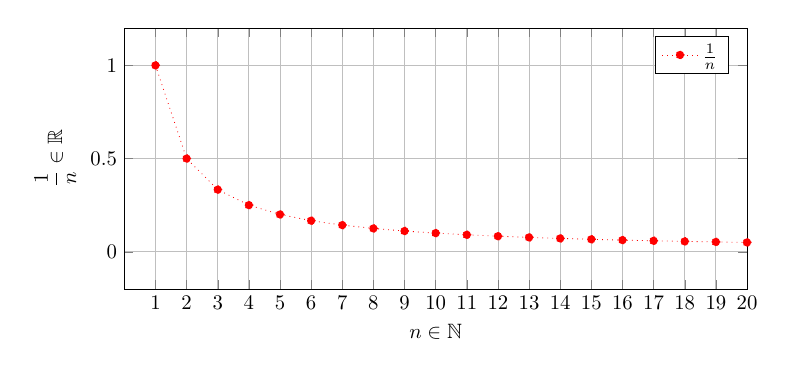
\begin{tikzpicture}[scale=.75]
	\begin{axis}[
		xlabel={$n \in \mathbb{N}$},
		ylabel={$\displaystyle\frac{1}{n}\in\R$},
		ymin=-.2, ymax=1.2,
		xmin=0, xmax=20,
		xtick={1,2,...,20},
		ytick={0,0.5,1},
		grid=major,
		width=\textwidth,
		height=6cm,
		domain=1:20,
		samples=20,
		legend pos=north east
		]
		% Plot points for 1 - 1/n
		%		\addplot[line width=.25mm, only marks, red, mark=x] plot (\x, 1 - 1/\x);
		\addplot[red, mark=*, dotted, mark options={fill=red}] plot (\x, 1/\x);
		\addlegendentry{$\frac{1}{n}$};
		
		% Draw horizontal line showing upper bound (y=1)
%		\addplot[dashed, magenta, line width=.5mm] coordinates {(0,1) (30,1)};
%		\node[magenta] at (axis cs: 3,1.1) {Upper Bound $1$};
		
		% Draw horizontal line showing lower bound (y=0)
%		\addplot[dashed, cyan, line width=.5mm] coordinates {(0,0) (30,0)};
%		\node[cyan] at (axis cs: 3,-0.1) {Lower Bound $0$};	
	\end{axis}
\end{tikzpicture}
	\end{center}
	\begin{proof}
		\textcolor{blue}{Let $\varepsilon>0$}. By the Archimedean property, we obtain \[
		\textcolor{blue}{\exists N_\epsilon\in\N}\quad \text{s.t.}\quad 1<\varepsilon\cdot N_\epsilon,\ \ie,\ \frac{1}{N_\epsilon}<\varepsilon.
		\] \textcolor{blue}{Assume that $n\geq N_\epsilon$ then} \[
		\textcolor{blue}{\abs{a_n-0}}=\abs{\frac{1}{n}}=\frac{1}{n}\leq\frac{1}{N_\epsilon}
		\textcolor{blue}{<\varepsilon}.
		\] Hence $\displaystyle\lim\limits_{n\to\infty}\frac{1}{n}=0$.
	\end{proof}
\end{example*}

\begin{example*}
	Consider the sequence defined by $b_n=1-(-1)^n$ for all $n\in\N$. Prove that $b_n$ does not converge. 
	\begin{center}
		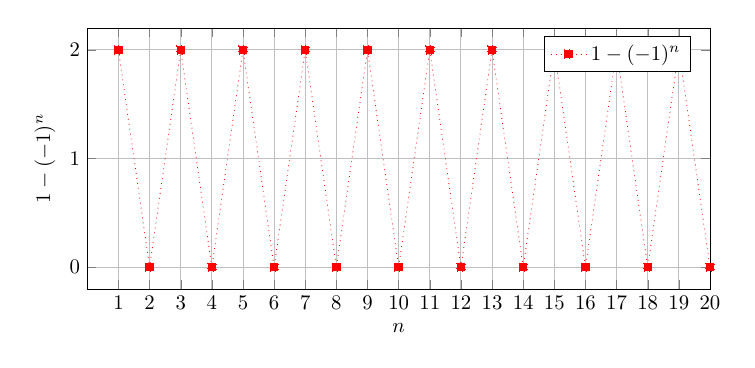
\begin{tikzpicture}[scale=.75]
	\begin{axis}[
		xlabel={$n$},
		ylabel={$1-(-1)^n$},
		ymin=-.2, ymax=2.2,
		xmin=0, xmax=20,
		xtick={1,2,...,20},
		ytick={0,1,2},
		grid=major,
		width=\textwidth,
		height=6cm,
		domain=1:20,
		samples=20,
		legend pos=north east,
		]
		\addplot[red, mark=square*, dotted, mark options={fill=red}] {1 - (-1)^x};
		\addlegendentry{$1-(-1)^n$};
		
		% Draw horizontal line showing upper bound (y=1)
		%		\addplot[dashed, magenta, line width=.5mm] coordinates {(0,1) (30,1)};
		%		\node[magenta] at (axis cs: 3,1.1) {Upper Bound $1$};
		
		% Draw horizontal line showing lower bound (y=0)
		%		\addplot[dashed, cyan, line width=.5mm] coordinates {(0,0) (30,0)};
		%		\node[cyan] at (axis cs: 3,-0.1) {Lower Bound $0$};	
	\end{axis}
\end{tikzpicture}
	\end{center}
	\begin{proof}
		Suppose that $\set{b_n}_{n=1}^\infty$ converges to $\beta\in\R$. \textcolor{blue}{Let $\varepsilon\in\intoo{0,2}$}. Then if $n\geq N_\varepsilon$, \begin{align*}
			\abs{b_n-\beta}&=\abs{b_n-b_{n+1}+b_{n+1}-\beta} \\
			&\leq\abs{b_n-b_{n+1}}+\abs{b_{n+1}-\beta} \\
			&=2+\abs{b_{n+1}-\beta}
		\end{align*}
	\end{proof}
\end{example*}

\newpage

\defbox[Absolute Value in Reals]{\begin{definition*}
	Let $x\in\R$. A \textbf{absolute value} $\abs{x}$ of $x$ is defined by \[
	\abs{x}:=\begin{cases}
		x &:x\geq 0\\
		-x &:x<0
	\end{cases}
	\]
\end{definition*}}
\probox{\begin{proposition*}
	Let $x,y\in\R$. \begin{enumerate}[\normalfont(a)]
		\item $\abs{x}=\abs{-x}=\sqrt{x^2}$
		\item $\abs{xy}=\abs{x}\abs{y}$
		\item For each $r>0$, \[
		\abs{x}<r\iff -r<x<r
		\]
		\item  \[
		\delta<\abs{x}\iff \delta<x\ \text{or}\ x<-\delta
		\]
		\item $-\abs{x}\leq x\leq \abs{x}$
		\item (Triangle Inequality) \[
		\abs{x+y}\leq\abs{x}+\abs{y}
		\]
	\end{enumerate}
\end{proposition*}}
\begin{proof}
	\begin{enumerate}[(a)]
		\item 
	\end{enumerate}
\end{proof}

\defbox[Boundedness of Sequence]{\begin{definition*}
	Let $\set{a_n}$ is a real sequence. $\set{a_n}$ is said to be \textbf{bounded} when \[
		\exists M\in\R\ \text{such that}\ \forall n\in\N,\ \abs{a_n}\leq M.
		\]
\end{definition*}}

\probox[]{\begin{proposition*}
	A convergent sequence is bounded.
\end{proposition*}}
\begin{proof}
	Let $\lim\limits_{n\to\infty}a_n=L$. For $\varepsilon=1$, $\exists N\in\N$ such that $n\geq N\implies\abs{a_n-L}<1$. Then we see that \[
	\abs{a_n}=\abs{a_n-L+L}\leq\abs{a_n-L}+\abs{L}<1+\abs{L}.
	\] Let $M:=\max\set{\abs{a_1},\abs{a_2},\dots,\abs{a_{N-1}},1+\abs{L}}$. Then \[
	\abs{a_n}\leq M
	\] for all $n\in\N$. That is, $\set{a_n}$ is bounded.
\end{proof}
%\begin{tikzpicture}[scale=2]
%	\begin{axis}[
%		title=Example using the mesh parameter,
%		hide axis,
%		colormap/cool,
%		]
%		\addplot3[
%		mesh,
%		samples=50,
%		domain=-8:8,
%		]
%		{sin(deg(sqrt(x^2+y^2)))/sqrt(x^2+y^2)};
%		\addlegendentry{\(\frac{sin(r)}{r}\)}
%	\end{axis}
%\end{tikzpicture}
\newpage



\vfill
\begin{thebibliography}{9}
	\bibitem{advanced_calc_c}
	수학의 즐거움, Enjoying Math. ``수학 공부, 기초부터 대학원 수학까지, 6. 해석학 개론 (c) 수열의 수렴성.'' YouTube Video, 26:29. Published 
	September 20, 2019. URL: \url{https://www.youtube.com/watch?v=jwLfzJyIxmU}.
	\bibitem{advanced_calc_d}
	수학의 즐거움, Enjoying Math. ``수학 공부, 기초부터 대학원 수학까지, 7. 해석학 개론 (d) 극한 정리'' YouTube Video, 26:46. Published 
	September 26, 2019. URL: \url{https://www.youtube.com/watch?v=1TRD34QbIaw}.
\end{thebibliography}

%\newpage
%\appendix
\end{document}
